\normaltrue
\correctionfalse

%\UPSTIidClasse{11} % 11 sup, 12 spé
%\newcommand{\UPSTIidClasse}{12}

\exer{Roue avant de GC10 -- V8 $\star$ \label{A5:05:86}}
\setcounter{question}{0}
%\UPSTIcompetence[2]{A5-05}
%\UPSTIcompetence[2]{A5-04}

\index{Compétence A5-05}
\index{Compétence A5-04}

\index{GPS}
\index{Spécification géométrique des produits}
\index{Roue motrice}

\ifcorrection
\else
\marginnote{\textbf{Pas de corrigé pour cet exercice.}}
\fi

\section*{Mise en situation}
\ifprof
\else
\fi

On s'intéresse à la roue avant et au pivot de roue d'une voiture de course et plus particulièrement au moyeu de roue.

\begin{center}
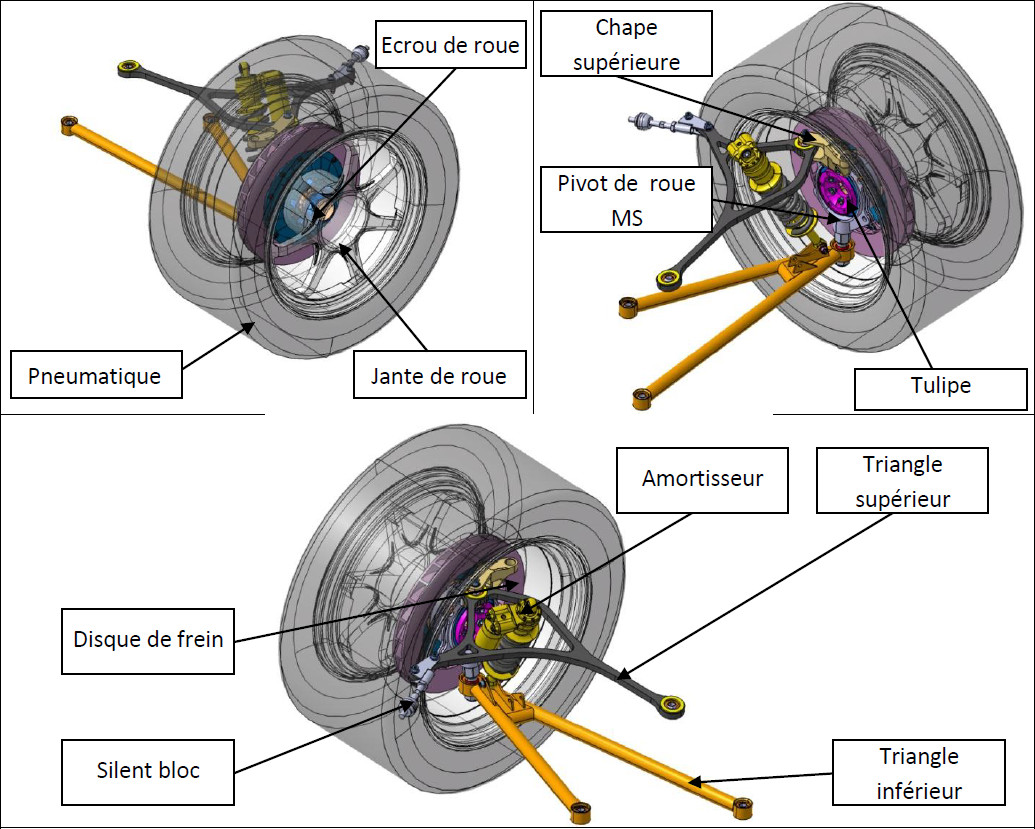
\includegraphics[height=8.5cm]{86_fig_02}
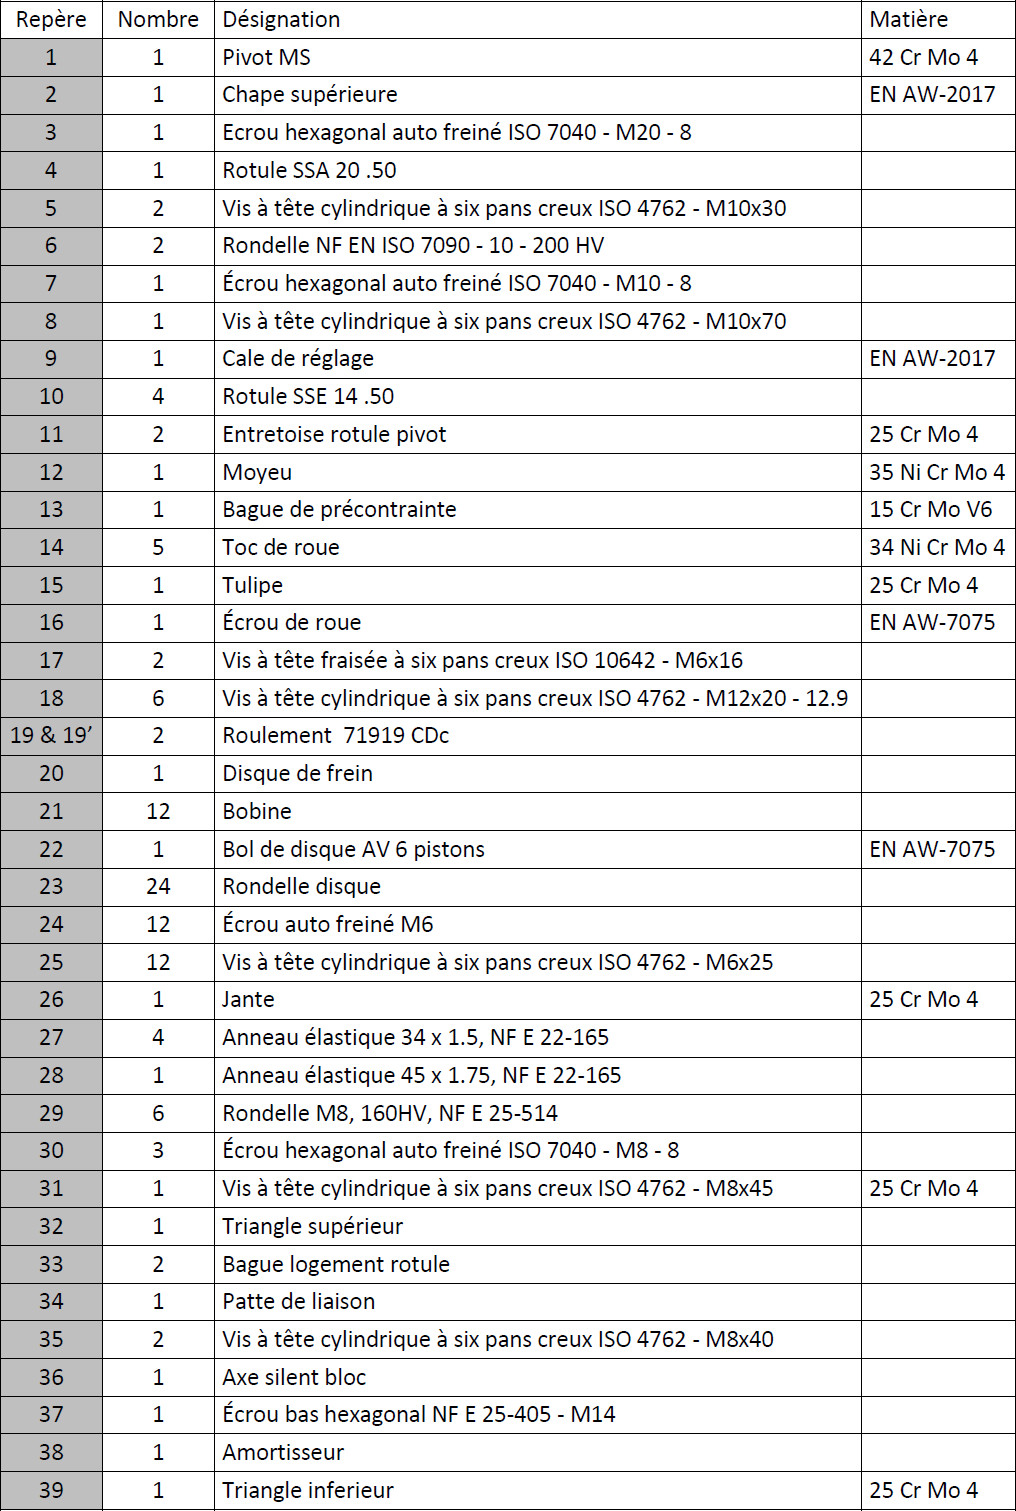
\includegraphics[height=8.5cm]{86_fig_03}
\end{center}

Le plan d'ensemble au verso montre l'assemblage du moyeu avec les autres constituants. 
\begin{marginfigure}
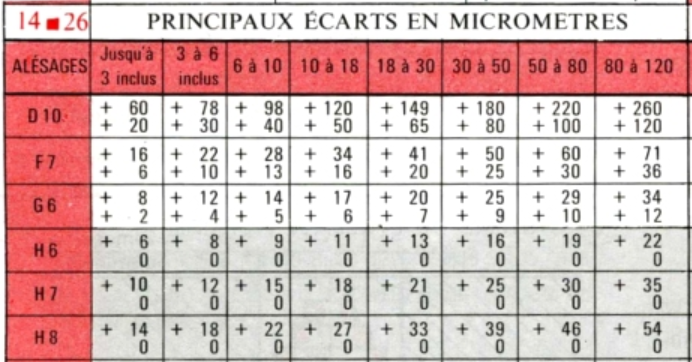
\includegraphics[width=\linewidth]{86_fig_04}
\end{marginfigure}

\subsection*{Analyse des spécifications géométriques et dimensionnelles}




%\begin{minipage}[c]{.6\linewidth}
\question{Expliquer quelle(s) fonction(s) du produit justifie l'existence des spécifications suivantes :
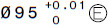
\includegraphics[width=2cm]{86_gps_01} et 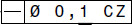
\includegraphics[width=2cm]{86_gps_02}.}


\question{Décrire les spécifications suivantes :
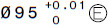
\includegraphics[height=.6cm]{86_gps_01}, 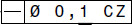
\includegraphics[height=.6cm]{86_gps_02}, 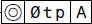
\includegraphics[height=.6cm]{86_gps_03}, 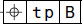
\includegraphics[height=.6cm]{86_gps_04} et 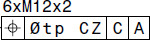
\includegraphics[height=.7cm]{86_gps_05}.}

\question{Quelle serait la conséquence d'un ajout du modificateur du maximum de matière sur l'intervalle de tolérance de la spécification de coaxialité ? sur l'élément de référence ?}
%
%\end{minipage} \hfill
%\begin{minipage}[c]{.38\linewidth}
%
%\begin{center}
%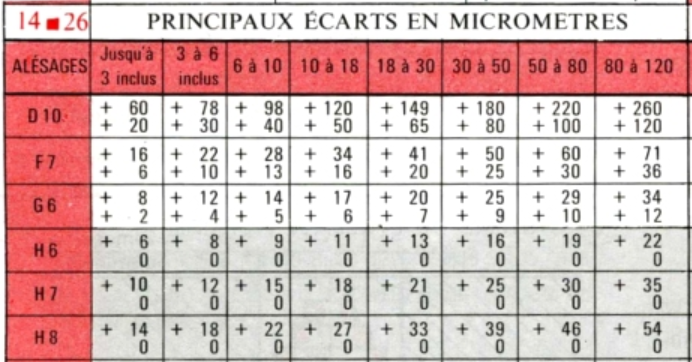
\includegraphics[width=.9\linewidth]{86_fig_04}
%\end{center}
%\end{minipage}
\subsection*{Analyse des procédés de fabrication}
\question{Donner l'ensemble des moyens de fabrications ayant mené à la réalisation du moyeu de roue.}

\question{Proposer une gamme de fabrication permettant de réaliser le moyeu.}

%\end{multicols}




%%\begin{center}
%%\rotatebox{270}{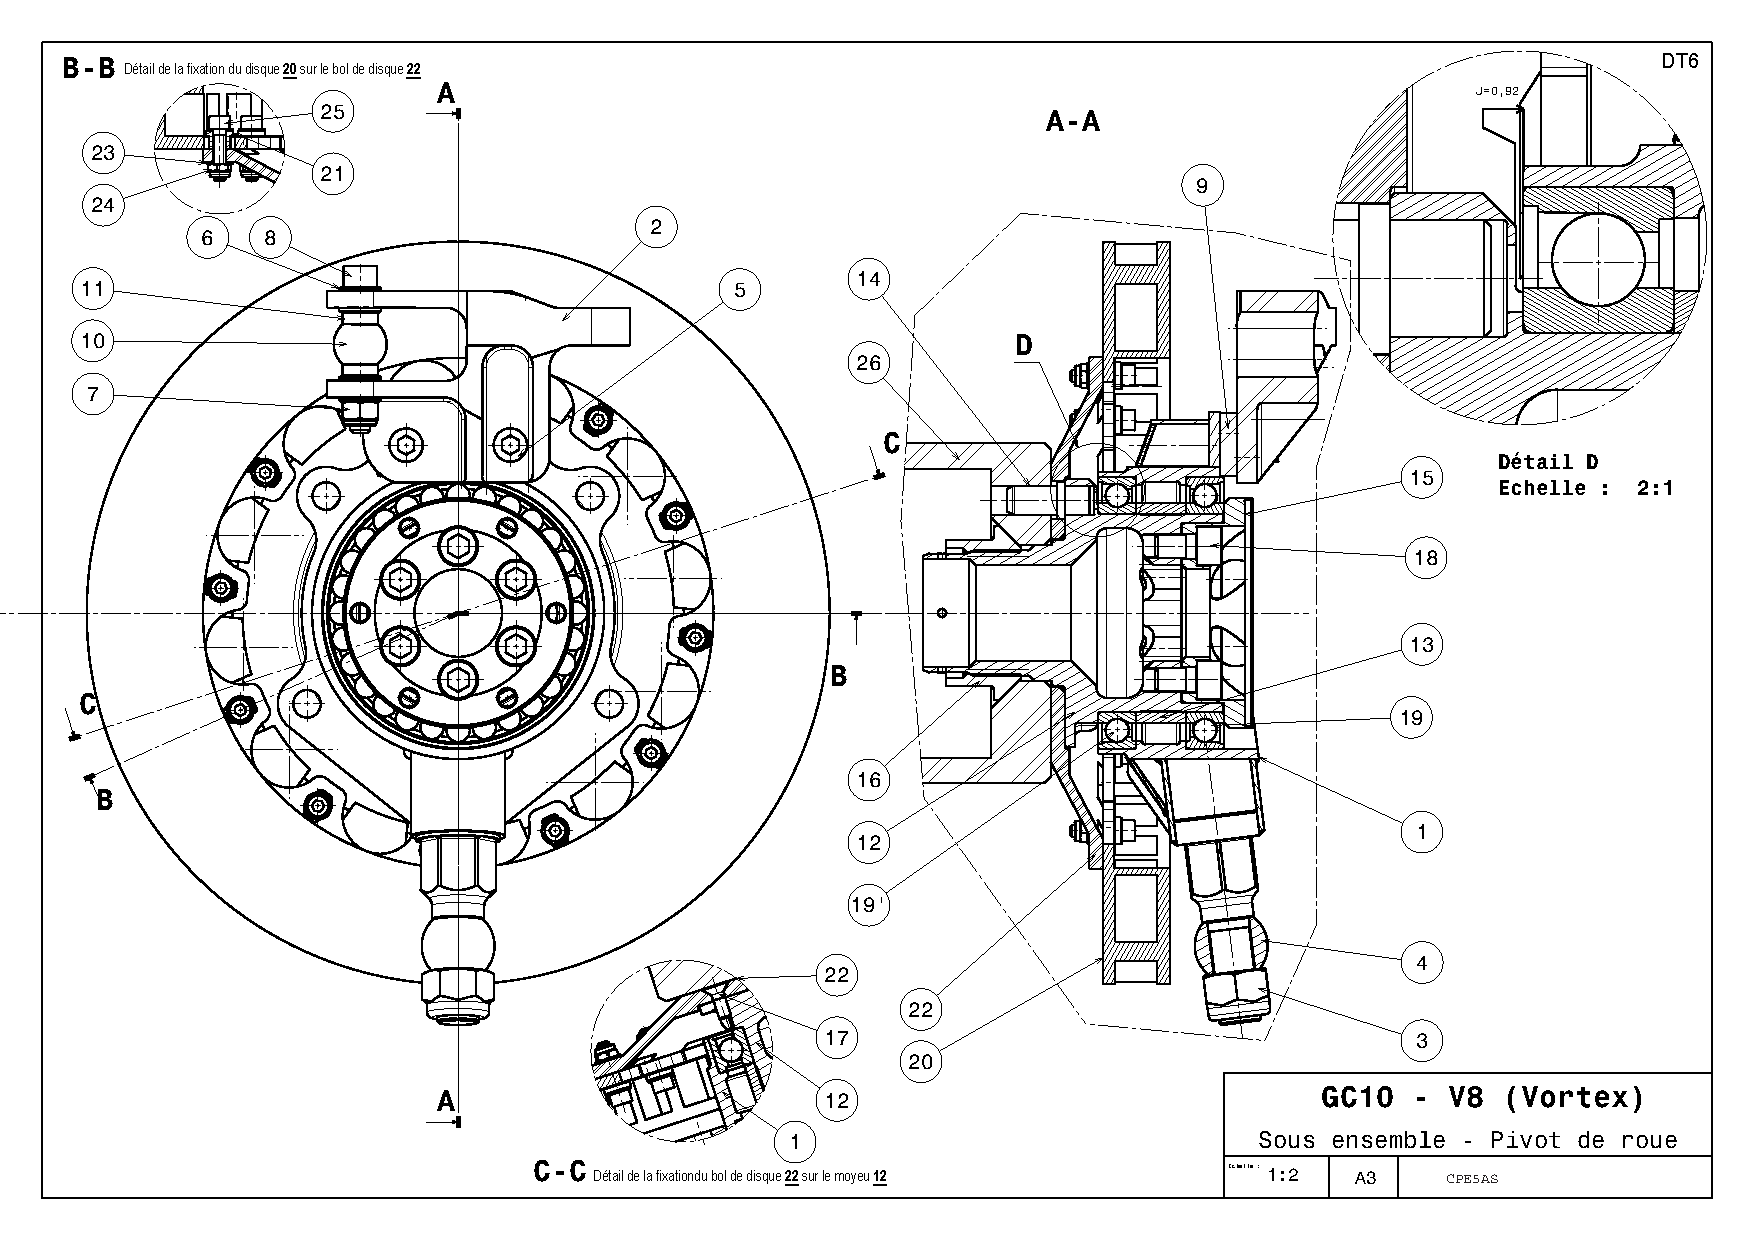
\includegraphics[height=\linewidth]{86_plan_01}}
%%
%%%{\includegraphics[width=\linewidth]{86_fig_06}}
%%\end{center}

\begin{figure*}[!h]
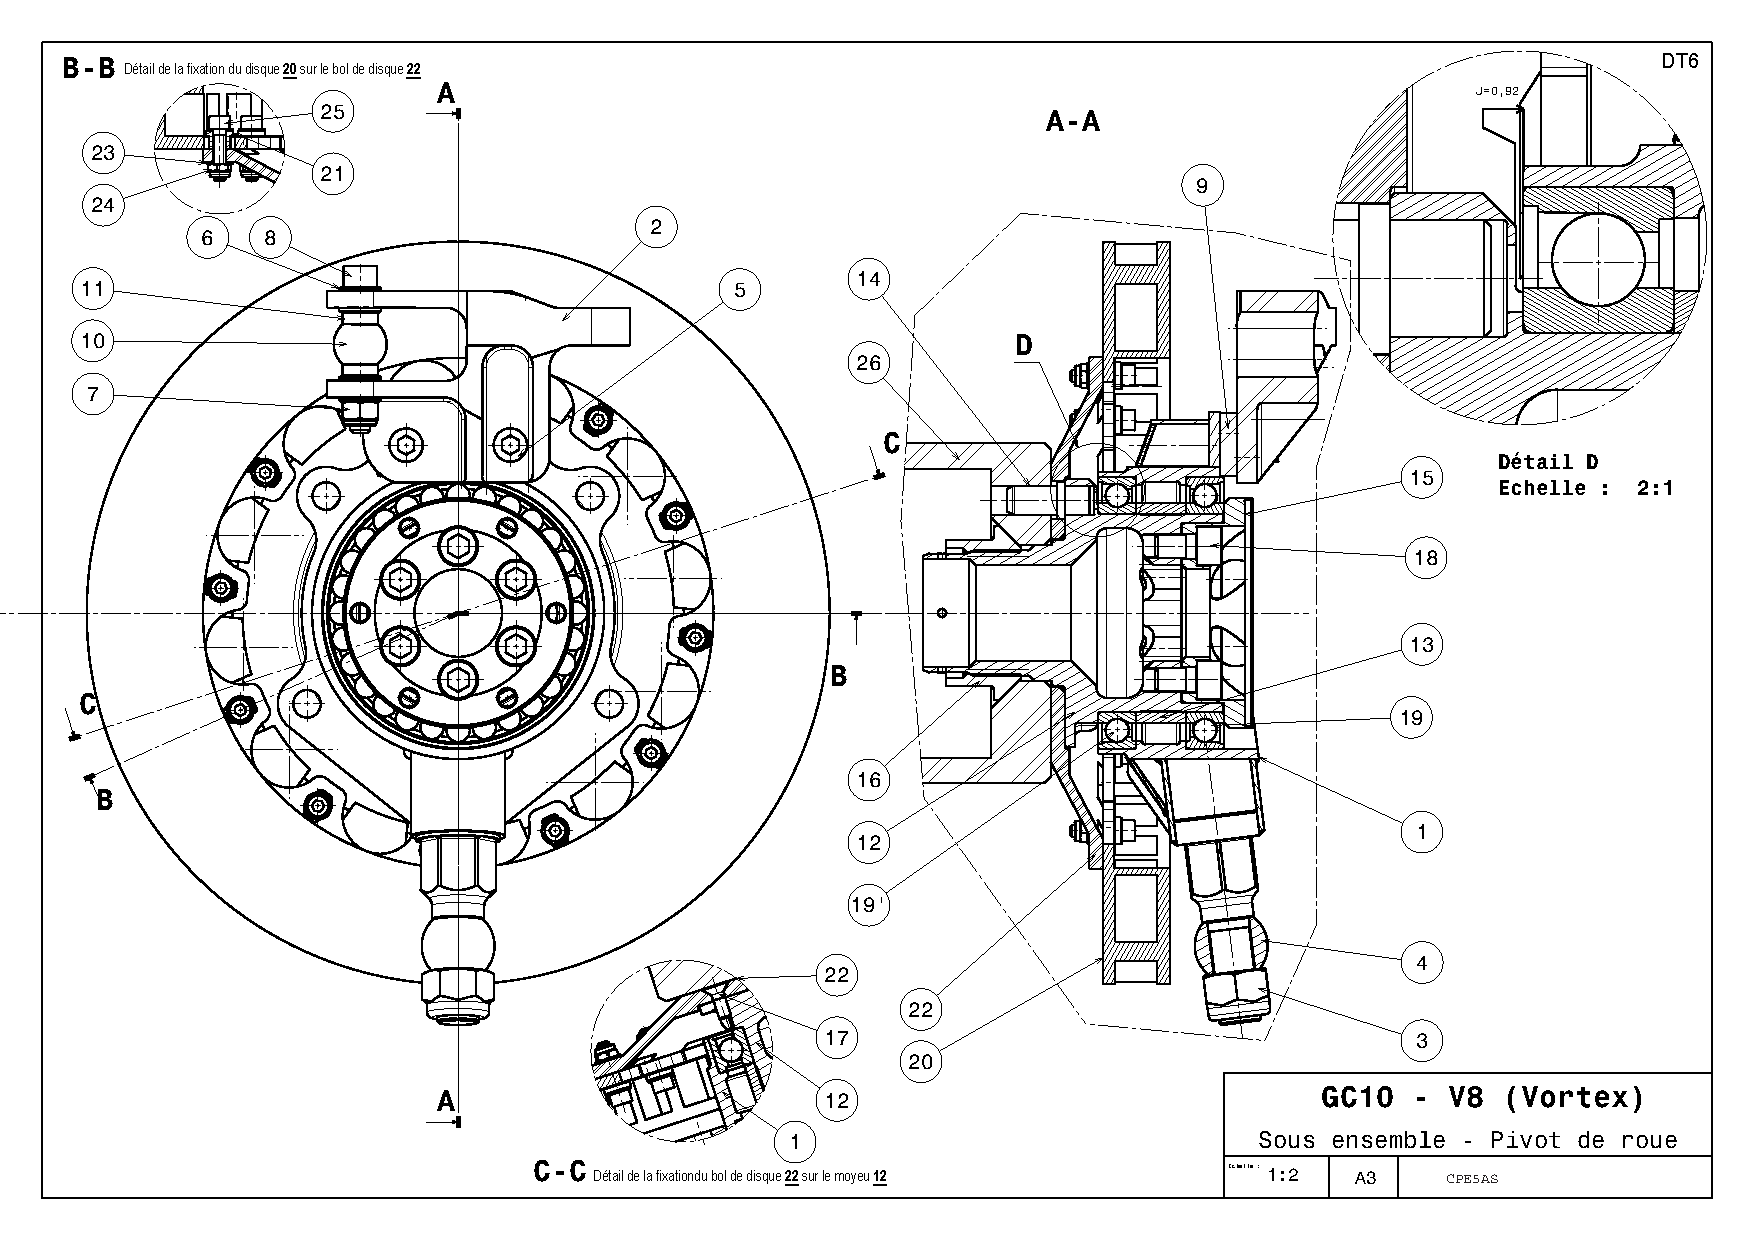
\includegraphics[width=\linewidth]{86_plan_01}
\end{figure*}

\begin{figure*}[!h]
\centering
\rotatebox{270}{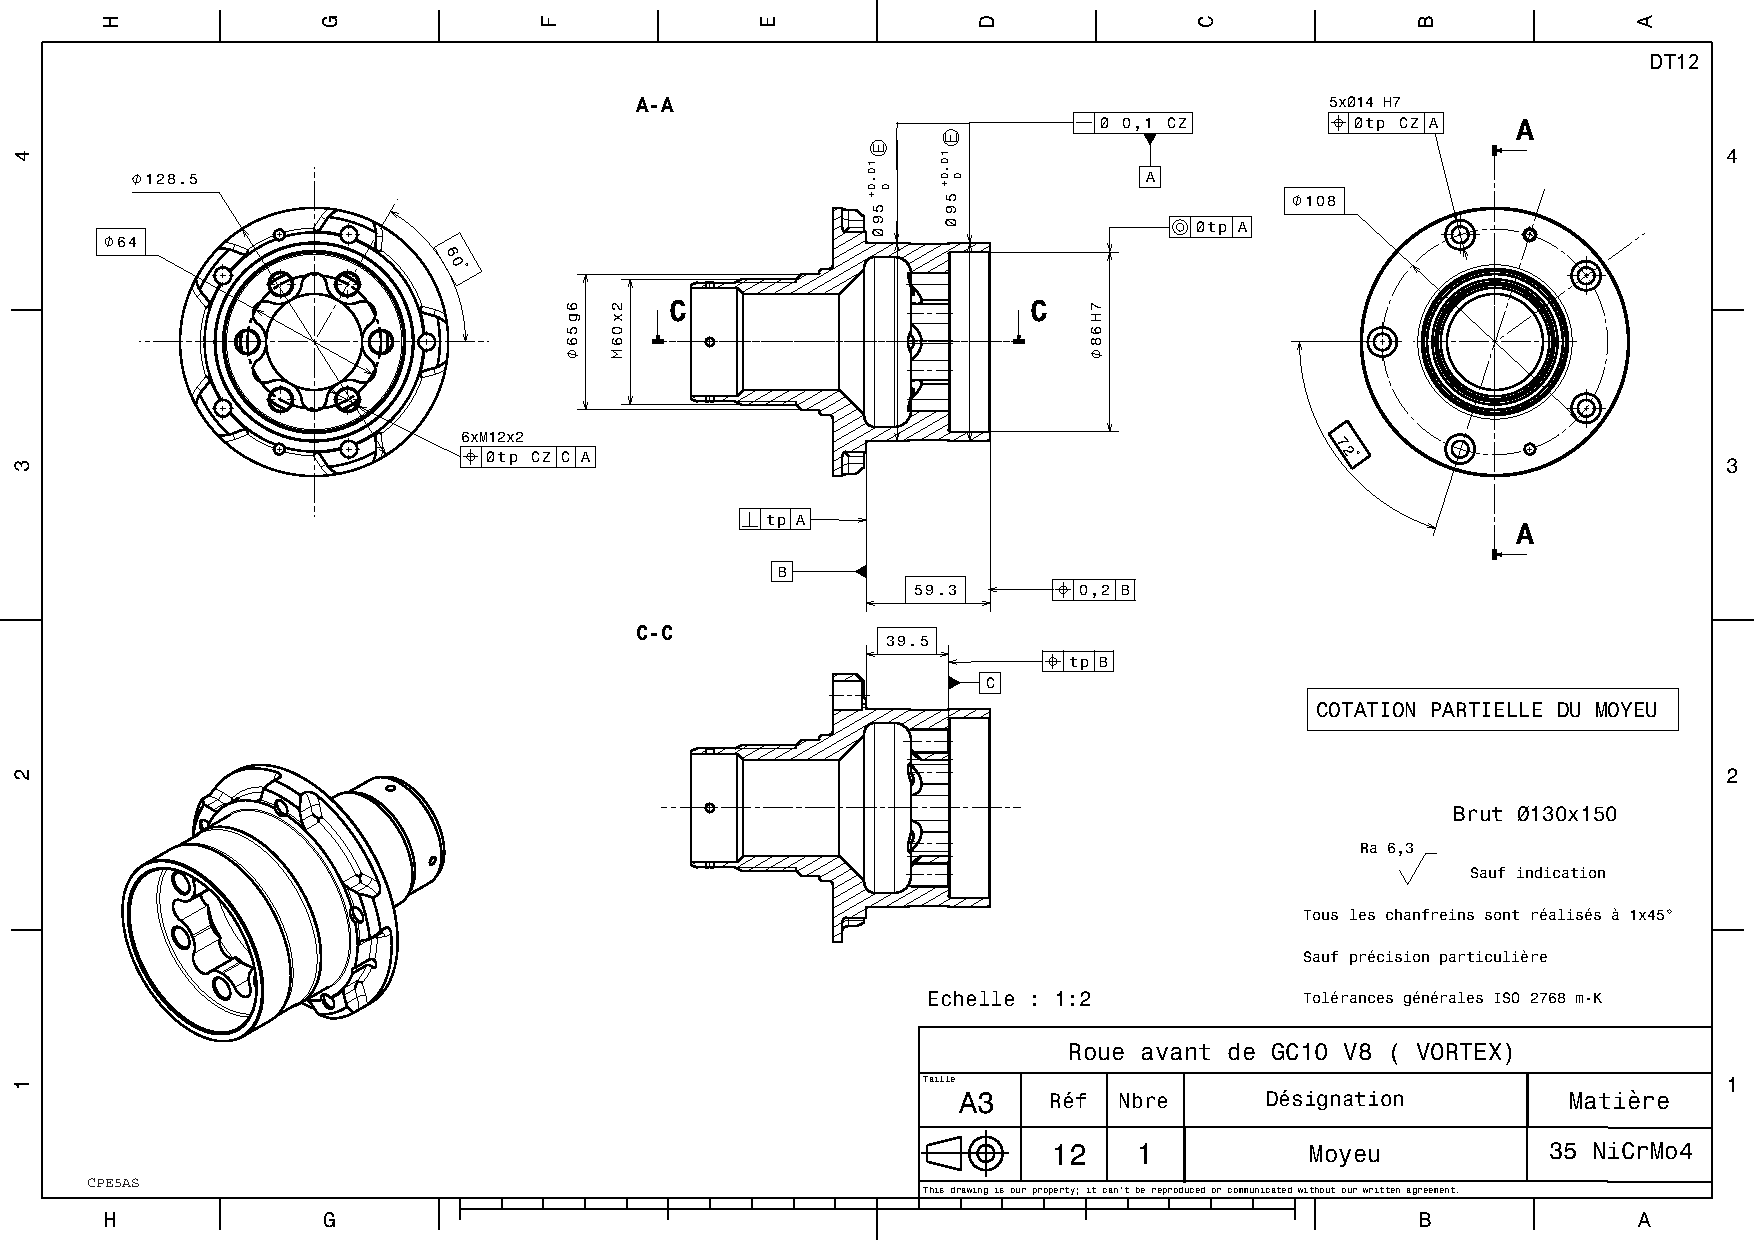
\includegraphics[height=1.3\linewidth]{86_plan}}
%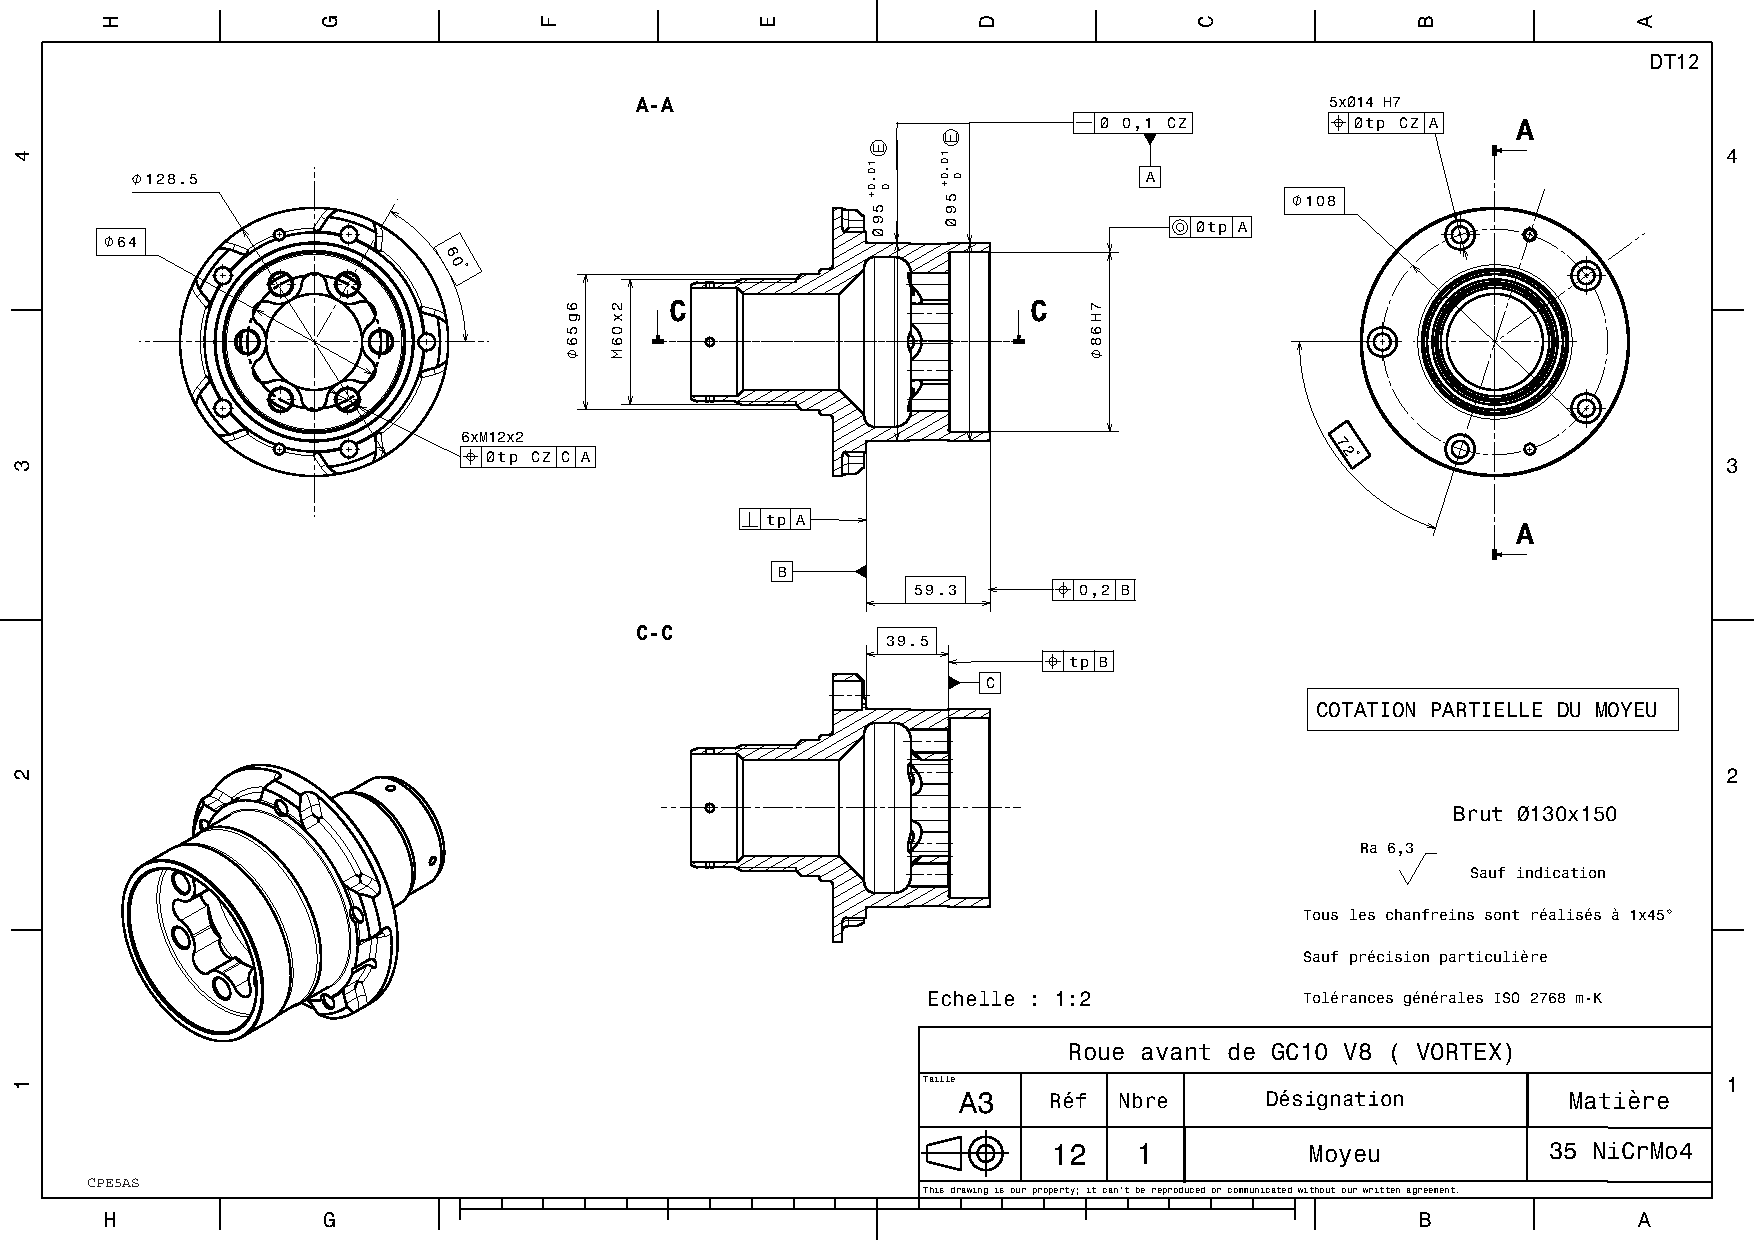
\includegraphics[width=\linewidth]{86_plan}

%{\includegraphics[width=\linewidth]{86_fig_06}}
\end{figure*}


\ifprof
\else
\begin{flushright}
\footnotesize{Corrigé  voir \ref{A5:05:86}.}
\end{flushright}%
\fi 